\documentclass[11pt,a4paper]{article}

\usepackage[utf8]{inputenc} 
\usepackage[T1]{fontenc} 
\usepackage{lmodern}
\usepackage[margin=2cm]{geometry}
\usepackage[german]{babel}
\usepackage{array}
\setlength{\parindent}{0pt}
\setlength{\parskip}{1ex plus 0.5ex minus 0.5ex}
\usepackage{amsmath} 
\usepackage{graphicx} 
\usepackage{booktabs}
\usepackage[colorlinks]{hyperref}
\usepackage{nicefrac}
\usepackage{gensymb}
\usepackage[usenames,dvipsnames,svgnames,table]{xcolor}
\usepackage{tcolorbox}
\usepackage[section]{placeins}

\hbadness=99999

\newenvironment{supbox}{\begin{tcolorbox}[colback=white,colframe=black,sharp corners,boxrule=.5pt]}{\end{tcolorbox}}
\begin{document}

{
\centering 
\large 
Physiklabor für Anf\"anger*innen \\
Ferienpraktikum im Sommersemester 2018 \\[4mm]
\textbf{\LARGE 
Versuch 31: Mischungsmethode in der Kalorimetrie
} \\[3mm]
(durchgef\"uhrt am 12.09.2018 bei Nico Strauß) \\
Andréz Gockel, Patrick M\"unnich\\
\today \\[10mm]
}

\tableofcontents

\pagebreak

\section{Ziel des Versuchs}


Der Versuch ist in drei Teile geteilt, welche dazu dienen, mit Hilfe einer geeigneten Wärmeenergiebilanz die Wärmekapazität zu bestimmen. Im Teil A kalibriert man das Messgerät und stellt das Programm, LabVIEW, ein. Im Teil B wird mittels Extrapolationsverfahren die Wärmekapazität des Kalorimeters bestimmt. Für die Messungen wurde ein Temperaturmessfühler, der durch einen DAQ zu einem Komputer verbunden wurde verwendet, dadurch konnten die Messdaten mittels dem Programm LabVIEW gespeichert werden. Im Teil C wurde die Wärmekapazität von zwei Festkörpern bestimmt. 

\section{Aufbau}

Der Messf\"uhler ist per Kabel an den PC gebunden, an dem LabVIEW l\"auft. Zwei mit Wasser gef\"ullte Beh\"alter sind vorhanden. Eins davon ist auf einer Heizplatte, das andere besteht aus Eiswasser.

\begin{figure}[ht!]
	\centering
	\fbox{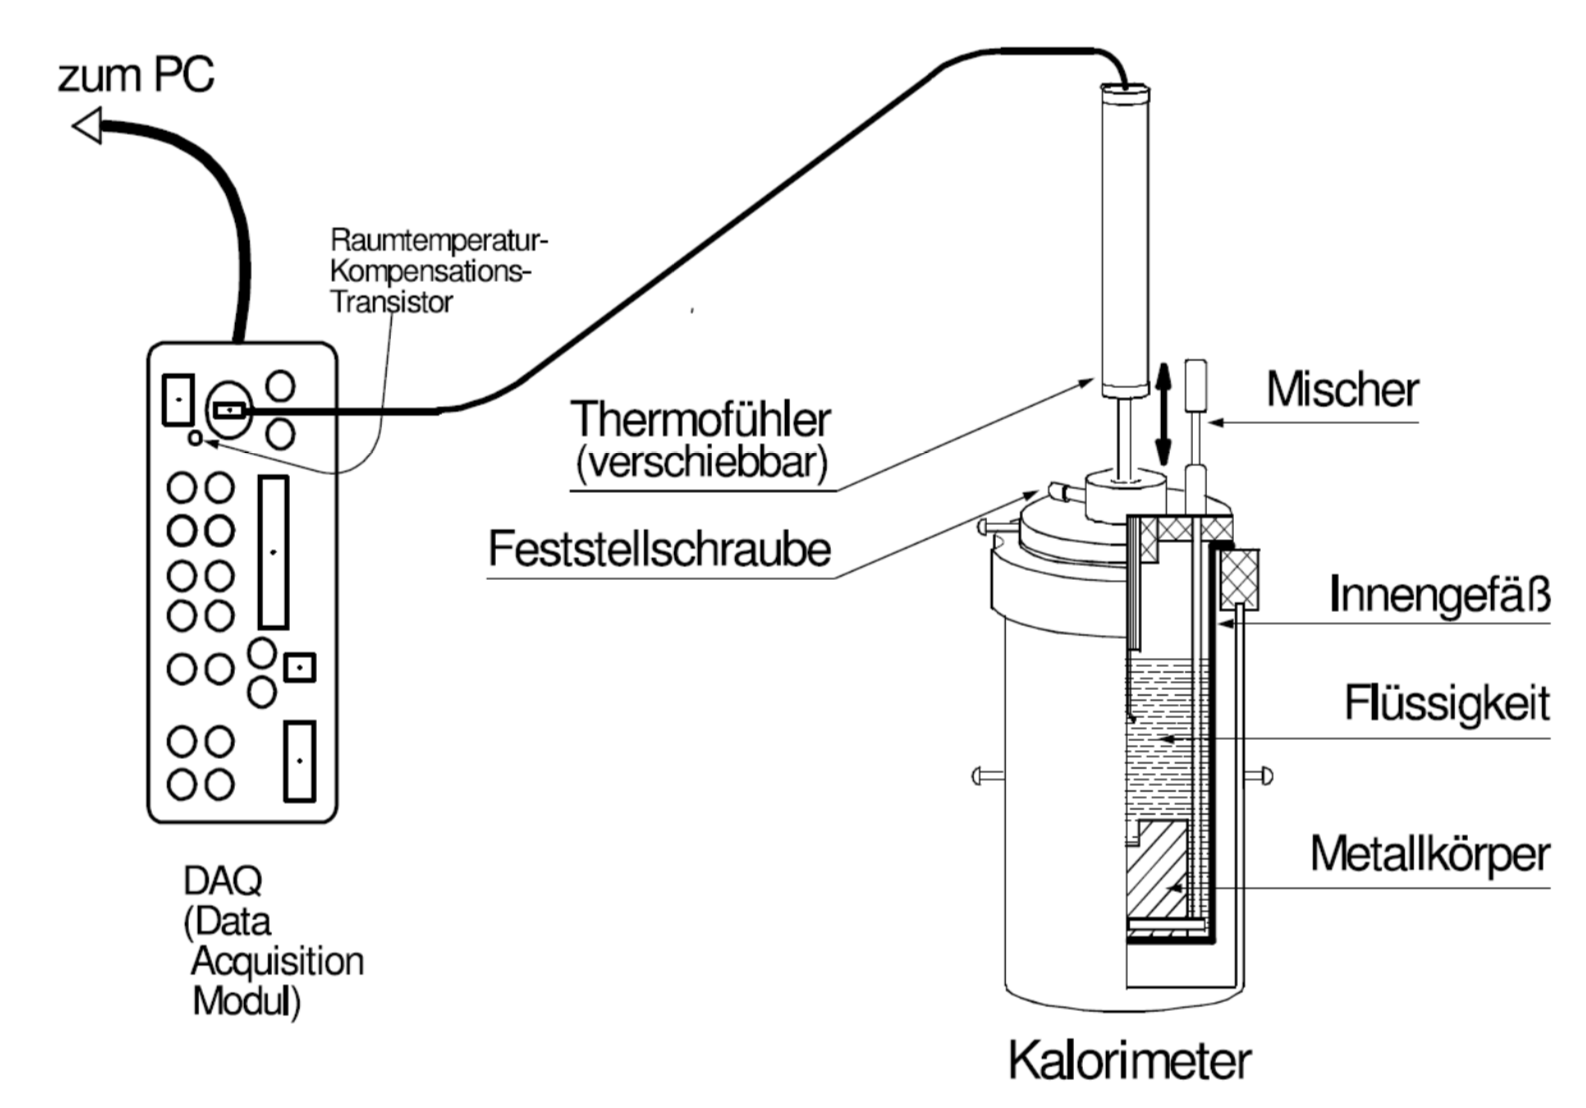
\includegraphics[width=0.7\textwidth]{Aufbaoo}}
  	\renewcommand\thefigure{B1}
	\caption{Der Aufbau}
	\label{Bild:1}
\end{figure}


\section{Auswertung und Fehleranalyse}

\subsection{Teil A - Kalibrierung des Messf\"uhlers}

\subsubsection{Durchf\"uhrung}
Zuerst vervollst\"andigt man LabVIEW, sodass die Temperatur und die Zeit nach der Messung in eine Datei abgespeichert wird.\\
Zur Kalibrierung wird das Ende des Messf\"uhlers, an dem gemessen wird, in das behitzte Wasserbad gesteckt und die Temperatur in LabVIEW an 100\celsius angepasst. Ist dies geschehen, so steckt man den Messf\"uhler in das Eiswasser und stellt dies auf 0\celsius ein.
\pagebreak
\subsubsection{Ergebnisse}
Bei der Kalibrierung wurden Schwankungen festgestellt. Bei dem kochenden Wasser lagen diese bei etwa 0.5\celsius, bei dem Eiswasser jedoch circa 2\celsius.\\
Dies liegt vermutlich aufgrund der kleinen Menge an Eiswasser, welche genutzt wurde, sowie auch daran, dass der Messf\"uhler nicht st\"andig im Wasser bzw. am Eis war, dar beides vorhanden ist. Ansonsten sind leichte Schwankungen nicht erstaunlich.

%Zur kalibrierung haben wir die Temperatur von Eiswasser und kochendem Wasser gemessen.
%
%Nach der vervollst\"andigung des Programms wurden die Temperaturen von kochendem Wasser und Eiswasser gemessen. Diese wurden so angepasst, dass sie jeweils circa $100\celsius$ und $0\celsius$ waren. Gro\ss e Schwankungen waren jedoch auff\"allig. Bei dem kochenden Wasser waren diese eher klein, bei etwa $0.5\celsius$. Bei dem Eiswasser waren Schwankungen von $2\celsius$ zu beobachten, vermutlich aufgrund dem Aufw\"armen des Wassers. Man sollte also bei den folgenden Messungen die Temperaturen kurz vor dem Mischen messen, da diese sich leicht \"andern k\"onnen.

\subsection{Teil B - Bestimmung von der Wärmekapazität des Kalorimeters: $C_{kal}$}

\subsubsection{Durchf\"uhrung}

Da genug Eiswasser nicht vorhanden ist, muss hier lauwarmes Wasser verwendet werden. Zuerst misst man die Temperaturen der beiden Wassermengen und wiegt sie, dann werden sie nacheinander in das Kalorimeter gef\"ullt und der Temperaturverlauf wird gemessen. Dies notiert man dann in ein Diagramm und eine Ausgleichskurve wird erstellt, mit der man die ware Mischtemperatur berechnet.

\subsubsection{Theorie}

Da das Kalorimeter und das Mischverfahren nicht vollkommen adiabatisch sind, also zur gleichen Zeit auch ein zus\"atzlicher Energieaustausch stattfindet und das Kalorimeter auch W\"arme aufnimmt, ist die Temperatur, die am Ende gemessen wird, nicht die wahre Mischtemperatur.\\
Zum Finden der wahren Mischtemperatur sucht man den Punkt, an dem man eine vertikale Gerade ziehen k\"onnte, welche die Fl\"achen zwischen der Kurve und den Geraden von jeweils der warmen und der kalten Wassermenge in zwei gleich gro\ss e Fl\"achen teilt.\\
Da unsere Werte einer $e$-Funktion \"ahneln, aber die Temperatur\"anderung linear verlaufen sollte, teilen wir unsere Ausgleichskurve in zwei Geraden auf, welche linear verlaufen.
Zum Berechnen dieses Punktes wird die folgende Gleichung genutzt:

\begin{equation}\tag{1}
\int\displaylimits_{t_{0}}^{t_2} f_M\ \mathrm{d}t - \int\displaylimits_{t_{0}}^{t_2} f_K\ \mathrm{d}t + f_{Add}= \int\displaylimits_{t_1}^{t_{0}} f_H\ \mathrm{d}t - \int\displaylimits_{t_1}^{t_{0}} f_M\ \mathrm{d}t.\label{bigint1}
\end{equation}

$f_K$ steht f\"ur die Gerade der Temperatur des kalten Wassers, $f_H$ f\"ur die Gerade der Temperatur des hei\ss en Wassers, $f_M$ f\"ur die Gerade der Mischung, welche $f_H$ schneidet, und $f_Add$ ist das Integral von der unteren Ausgleichsgerade der Mischung, welche $f_K$ schneidet. Die Integralgrenzen sind Zeiten, $t_0$ die gesuchte halbierende Zeit, $t_1$ der Schnittpunkt von $f_M$ mit $f_H$ und $t_2$ der Schnittpunkt von $f_M$ mit $f_K$. Da $f_{Add}$ wesentlich kleiner ist als die rechte Seite, wenn $f_{Add}$ bei $t_0$ w\"are, nehmen wir $f_{Add}$ als konstant an. Dies erleichtet uns sp\"ater das Aufl\"osen des Integrals. Alle Geraden sind in Form eines Polynoms ersten Grades:
%\begin{equation}
%f_M=a_Mx^2+b_Mx+c_M
%\end{equation}
\begin{equation}
f_{}=a_{}x+b_{}
\end{equation}
$f_{Add}$ sieht folgenderma\ss en aus:
\begin{equation}
f_{Add}=\int\displaylimits_{t_{3}}^{t_4}f_A\mathrm{d}t-\int\displaylimits_{t_{3}}^{t_4}f_K\mathrm{d}t,
\end{equation}
wobei $t_3$ und $t_4$ in diesem Fall 5\,s und 10\,s sind.

Integrieren wir und bringen die Gleichung in Form einer quadratischen Gleichung bez\"uglich dem gesuchten $t_0$, so k\"onnen wir folgenderma\ss en nach $t_0$ aufl\"osen:
\begin{equation}
t_{0_{1/2}}=\frac{-B\pm\sqrt{B^2-4AC}}{2A},\label{abc1}
\end{equation}
Hier sind unsere Variablen

\[
A=\frac{a_K}{2}-\frac{a_H}{2}
\]

\[
B=b_K-b_H
\]

\[
C=a_M\frac{t_2^2}{2}+b_Mt_2-a_K\frac{t_2^2}{2}-b_Kt_2+f_{Add}+a_H\frac{t_1^2}{2}+b_Ht_1-\frac{a_m}{2}t_1^2-b_mt_1.
\]

Die wahre Mischungstemperatur $T_M$ kann dann einfach von den Werten von $f_M$ abgelesen werden.

Um hieraus die W\"armekapazit\"at $C_{Kal}$ des Kalorimeters zu bestimmen wird
\begin{equation}
C_{Kal}=c_w(m_K\beta-m_H)\label{ck1}
\end{equation}

mit 
\[
\beta=\frac{T_M-T_K}{T_H-T_M}
\]
verwendet. Die Variablen stehen f\"ur folgende Werte:
\begin{itemize}
\item{$c_w$ die W\"armekapazit\"at von Wasser}
\item{$m_K$ die Masse des kalten Wassers}
\item{$m_H$ die Masse des warmen Wassers}
\item{$T_M$ die Mischungstemperatur}
\item{$T_K$ die Temperatur des kalten Wassers}
\item{$T_H$ die Temperatur des warmen Wassers}
\end{itemize}



\subsubsection{Auswertung}

Aufgrund eines Messfehlers, aufgrund dessen die Messung zwischen der Temperaturmessung des warmen Wassers und des Kalorimeters unterbrochen wurde, wurde angenommen, dass ein 15\,s Zeitraum zwischen den Messungen lag.

Mithilfe von (\ref{abc1}) bekommen wir zwei Ergebnisse f\"ur $t_0$. Das gr\"o\ss ere Ergebnisse ist klar das sinnvollere, da das kleinere keine gleich gro\ss en Fl\"achen liefert.

Unser $T_M$ liegt also bei ($59\pm2$)\celsius. Der Graph hierzu ist im Anhang zu finden.

Die Temperatur des kalten Wassers vor dem Eintauchen betrag $(22\pm1)$\celsius \ und die des warmen Wassers $(80\pm1)$\celsius. Die Masse des warmen Wassers war $(339.84\pm0.05)$\,g und die des kalten Wassers $(221.80\pm0.05)$\,g. Mit (\ref{ck1}) bekommen wir als Wert f\"ur $C_{Kal}$ $(190\pm90)\,\nicefrac{\mathrm{J}}{\mathrm{K}}$.

Die Berechnung des Fehlers wird durchgef\"uhrt mit:

\begin{equation}
s_x=\sqrt{\frac{1}{n-1}\sum_{i=1}^n(x_i-\overline{x})^2}\label{uncertainty1}
\end{equation}





\subsubsection{Diskussion}

Aufgrund des in der Auswertung angesprochenen Messfehlers ist die Temperatur des warmen Wassers geraten, was die wahre Mischtemperatur stark beeinflusst. Ist der Zeitraum zu gro\ss z\"ugig angenommen, so liegt die wahre Mischtemperatur h\"oher, andersrum wenn der Zeitraum zu klein angenommen ist. Der Grund f\"ur den starken Einfluss ist, dass in (\ref{abc1}) der Wert f\"ur $t_1$ sich dadurch \"andert, welcher in $C$ enthalten ist. Schaut man sich das Integral (\ref{bigint1}) an, so ist offensichtlich, dass $t_2$ als Integralgrenze bei beiden Integralen auf der linken Seite einen gro\ss en Einfluss hat.

Systematische Fehler hier sind, dass UNCERTAINTIES

\pagebreak

\subsection{Teil C - Bestimmung von der Spezifischen W\"armekapazit\"at von Festk\"orpern}

\subsubsection{Durchf\"uhrung}

Ein Festk\"orper wird im Wasserbad erhitzt, die Temperatur gemessen, und dann ins mit kalten Wasser gef\"ulltes Kalorimeter gef\"ullt. Dort wird wieder die Temperatur gemessen. Wie beim vorherigen Versuch wird hier wieder ein Diagram aufgezeichnet und mit einer Ausgleichskurve die Mischtemperatur gefunden. 

\subsubsection{Theorie}

Die Theorie hier gleicht der des vorherigen teils. Jedoch ist es hier aufgrund der Form der Messwerte im Diagram m\"oglich, in der Gleichung (\ref{bigint1}) den Term $f_{Add}$ wegzulassen. Dadurch ist in $C$ in (\ref{abc1}) nicht mehr n\"otig, den $f_{Add}$ Term hinzu zu addieren.

Zur Bestimmung der Mischtemperatur wird hier einfach folgende Gleichung nach $t_m$ aufgel\"ost und dann die Temperatur daraus abgelesen:

\begin{equation}
\int_{t_H}^{t_m}f_H\mathrm{d}t-\int_{t_H}^{t_m}f_M\mathrm{d}t=\int_{t_m}^{t_K}f_M\mathrm{d}t-\int_{t_m}^{t_K}f_K\mathrm{d}t\label{bigint2}
\end{equation}

Um aus der Mischtemperatur die spezifische W\"armekapazit\"at des K\"orpers zu bestimmen, wird die Formel (\ref{ck2}) verwendet.

\begin{equation}
c_K=\frac{m_Fc_F+C_{Kal}}{m_K}\beta\label{ck2}
\end{equation}

Hier ist $\beta$ definiert als
\[
\beta=\frac{T_M-T_F}{T_K-T_M}
\]
mit $T_M$ die Mischungstemperatur, $T_F$ die Temperatur der Fl\"ussigkeit und $T_K$ die Temperatur des Festk\"orpers. $m_F$ ist die Masse der Fl\"ussigkeit, $c_F$ die W\"armekapazit\"at der Fl\"ussigkeit, $C_{Kal}$ die W\"armekapazit\"at des Kalorimeters und $m_K$ die Masse des K\"orpers.

\subsubsection{Auswertung}

Die W\"armekapazit\"at unseres Kalorimeters haben wir im ersten Teil berechnet, also ist sie $(190\pm90)\,\nicefrac{\mathrm{J}}{\mathrm{K}}$. Die Masse der sich im Kalorimeter befindende Fl\"ussigkeit betr\"agt $(219.3\pm0.05)$\,g. Die spezifische W\"armekapazit\"at des Wassers betr\"agt $4182\,\nicefrac{\mathrm{J}}{\mathrm{kgK}}$. Die Temperatur des kalten Wassers innerhalb des Kalorimeters liegt bei $(20\pm0.4)$\celsius\ und die des Festk\"orpers vor dem Mischen $(71.97\pm0.4)$\celsius.

Laut unser aus (\ref{bigint2}) berechnetes $t_m$, welches bei $(29\pm0.5)$\,s liegt, ist unsere wahre Mischtemperatur $(44.4\pm0.4)$\celsius. Der hierzu geh\"orige Graph befindet sich wieder im Anhang.

Mit (\ref{ck2}) bekommen wir dann als Wert f\"ur unser $c_K$ $(1.40\pm0.12)\times10^4\,\nicefrac{\mathrm{J}}{\mathrm{kgK}}$. Unser Fehler wurde hier wieder mit (\ref{uncertainty1}) berechnet.

\subsubsection{Diskussion}

Bei diesem Teil war die Messproblematik des vorherigen Versuchsteils nicht mehr vorhanden. Jedoch gibt es immer noch einen Einfluss dessen aufgrund der Inklusion von $C_{Kal}$ in (\ref{ck2}).

Der Literaturwert der spezifischen W\"armekapazit\"at von METAL ist VALUE. Mit der Formel

\begin{equation}
t=\frac{|x_0-y|}{u_x}\label{abw}
\end{equation}

berechnen wir eine Abweichung von $t=ECKSDEE$ mit unserem gemessenen Wert. Dies liegt im Bereich von $t<2$, was Vertr\"aglichkeit der Werte impliziert. Es ist also wahrscheinlich, dass unser Festk\"orper aus METAL besteht.



\pagebreak

\section{Anhang}

%\begin{figure}[p]
%\centering
%\fbox{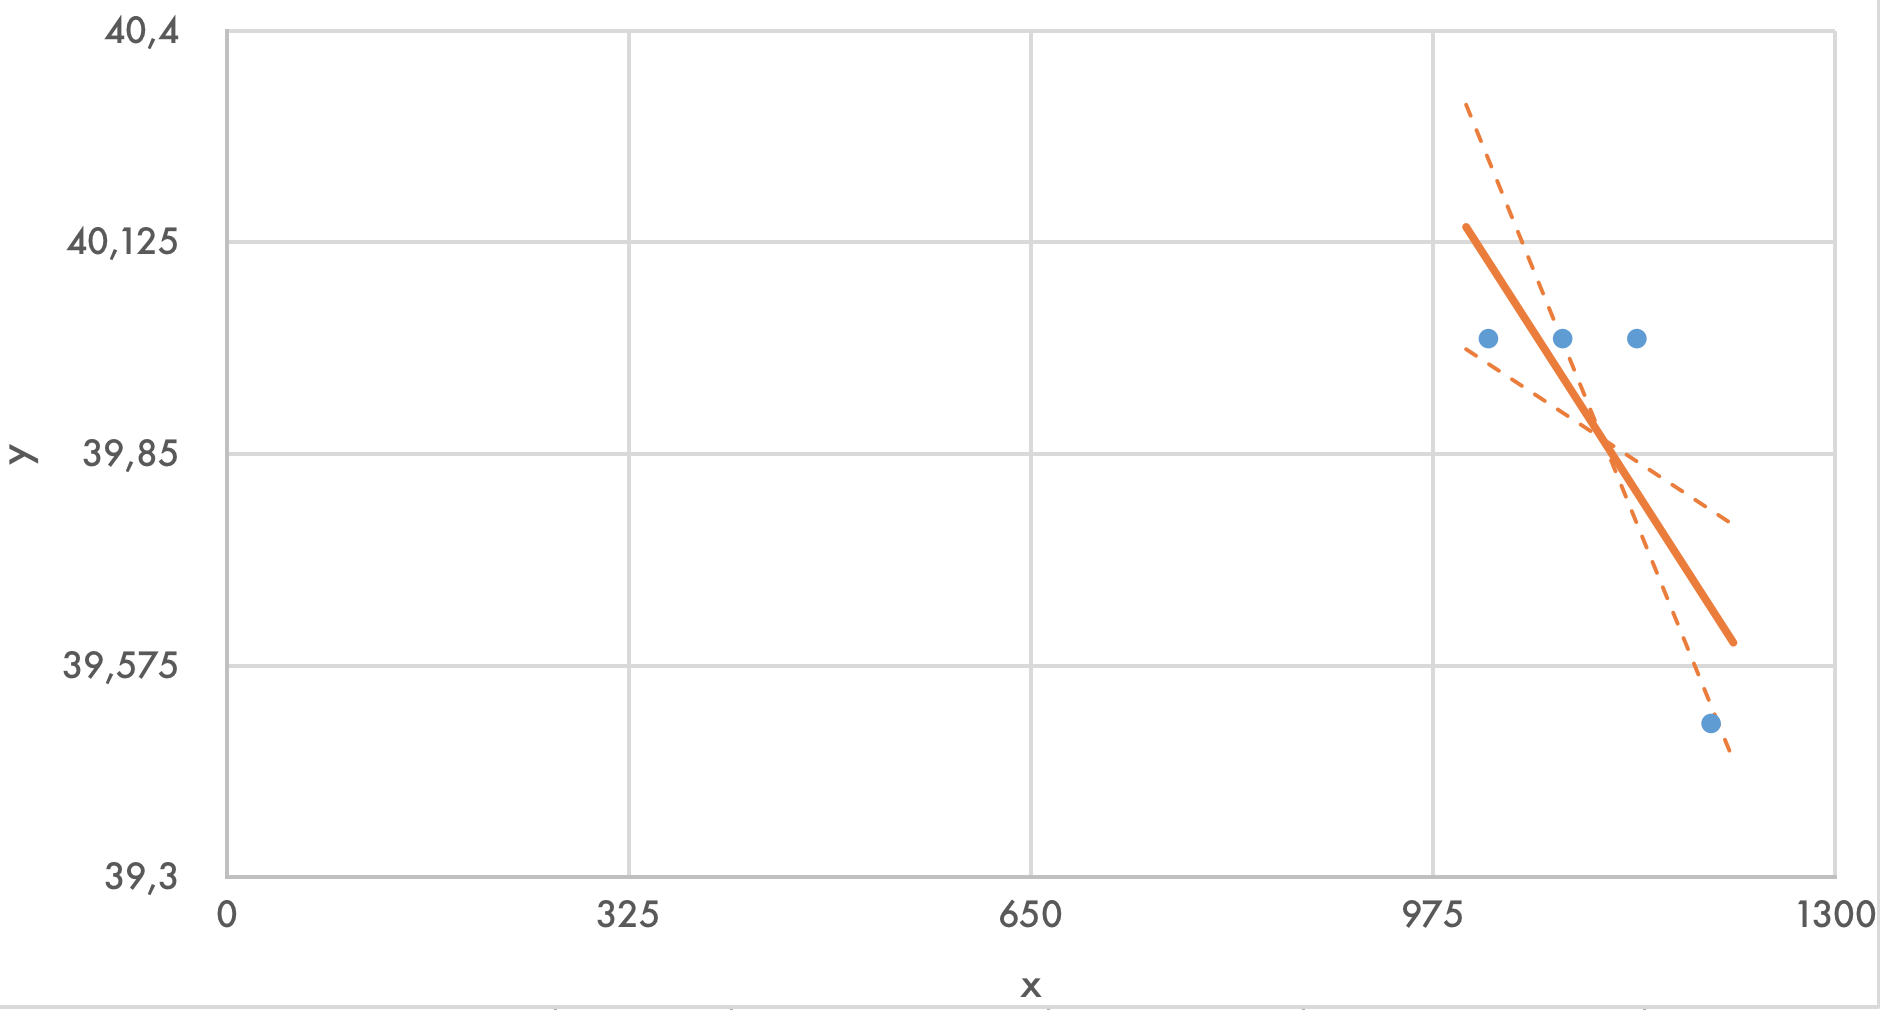
\includegraphics[width=0.7\textwidth]{extrapDia}}
%   \renewcommand\thefigure{A1}
%\caption{Extrapolation 2. Messreihe}
%\label{Dia:1}
%\end{figure}
%
%
%\begin{table}[p]
%	\centering
%	\rowcolors{2}{gray!10}{white}
%	\begin{tabular}{|r|l|}
%		\multicolumn{2}{c}{\textrm{Messreihe 1}} \\
%		\noalign{\global\arrayrulewidth=0.4mm}
%		\hline
%		\noalign{\global\arrayrulewidth=0.2mm}
%		\textrm{Rotationen }$n \pm 0.3$ & \textrm{Temperatur }$T \pm 0.05\celsius$\\
%		\hline
%		0 & 24 \\
%		10 & 24.1 \\
%		20 & 24.3 \\
%		30 & 24.5 \\
%		40 & 24.6 \\
%		50 & 24.8 \\
%		\hline
%	\end{tabular}
%	\renewcommand\thetable{T1}
%	\caption{Messreihe 1 für den ersten Versuchsteil}
%	\label{table:m1}
%\end{table}
%
%\begin{table}[p]
%	\centering
%	\rowcolors{2}{gray!10}{white}
%	\begin{tabular}{|r|l|}
%		\multicolumn{2}{c}{\textrm{Messreihe 2}} \\
%		\noalign{\global\arrayrulewidth=0.4mm}
%		\hline
%		\noalign{\global\arrayrulewidth=0.2mm}
%		\textrm{Rotationen }$n \pm 0.3$ & \textrm{Temperatur }$T \pm 0.05\celsius$\\
%		\hline
%		0 & 24.3 \\
%		5 & 24.3 \\
%		10 & 24.4 \\
%		15 & 24.5 \\
%		20 & 24.6 \\
%		25 & 24.7 \\
%		30 & 24.8 \\
%		35 & 24.9 \\
%		40 & 25 \\
%		45 & 25.1 \\
%		50 & 25.2 \\
%		55 & 25.2 \\
%		60 & 25.4 \\
%		65 & 25.5 \\
%		70 & 25.5 \\
%		75 & 25.6 \\
%		80 & 25.6 \\
%		85 & 25.7 \\
%		90 & 25.8 \\
%		95 & 26 \\
%		100 & 26 \\
%		\hline
%	\end{tabular}
%	\renewcommand\thetable{T2}
%	\caption{Messreihe 2 für den ersten Versuchsteil}
%	\label{table:m2}
%\end{table}
%
%\begin{table}[p]
%\centering
%$\begin{array}{rl}
%\multicolumn{2}{c}{\textrm{\underline{Unsicherheiten:}}}\\
%\textrm{Zeit: } & \pm 0.03 \textrm{s}\\
%\textrm{Temperatur: } & \pm 0.02 \textrm{\celsius}\\
%\textrm{Strom: } & \pm 0.03 \textrm{A}\\
%\textrm{Spannung: } & \pm 0.02 \textrm{V}
%\end{array}$
%\rowcolors{2}{gray!10}{white}
%\begin{tabular}{|c|c|c|c|}
%\multicolumn{4}{l}{Wasser 116.94(3)\,g}\\
%\hline
%$t$ in s & $T$ in $^\circ\textrm{C}$ & $I$ in A & $U$ in V \\
%\hline 
%0   & 22   & 1.5 & 14.9 \\
%60  & 22   & 1.5 & 14.9 \\
%120 & 23   & 1.5 & 14.9 \\
%180 & 24.5 & 0   & 0    \\
%240 & 26.3 & 0   & 0    \\ 
%300 & 26.5 & 0   & 0    \\ 
%360 & 26.5 & 0   & 0	\\ 
%$\vdots$ & $\vdots$ & $\vdots$ & $\vdots$ \\
%2280 & 26.4 & 0 & 0 \\
%\hline
%\end{tabular}
%\phantom{$\begin{array}{rl}
%\multicolumn{2}{l}{\textrm{\underline{Unsicherheiten:}}}\\
%\textrm{Zeit: } & \pm 0.03 \textrm{s}\\
%\textrm{Temperatur: } & \pm 0.02 \textrm{\celsius}\\
%\textrm{Strom: } & \pm 0.03 \textrm{A}\\
%\textrm{Spannung: } & \pm 0.02 \textrm{V}
%\end{array}$
%}
%\renewcommand\thetable{T4}
%\caption{1. Messwerte für Teil B}
%\label{tab:B1}
%\end{table}
%
%\begin{table}[p]
%\centering
%$\begin{array}{rl}
%\multicolumn{2}{l}{\textrm{\underline{Unsicherheiten:}}}\\
%\textrm{Zeit: } & \pm 0.03 \textrm{s}\\
%\textrm{Temperatur: } & \pm 0.02 \textrm{\celsius}\\
%\textrm{Strom: } & \pm 0.03 \textrm{A}\\
%\textrm{Spannung: } & \pm 0.02 \textrm{V}
%\end{array}$
%\rowcolors{2}{gray!10}{white}
%\begin{tabular}{|c|c|c|c|}
%\multicolumn{4}{l}{Wasser 113.42(3)\,g}\\
%\hline
%$t$ in s & $T$ in $^\circ\textrm{C}$ & $I$ in A & $U$ in V \\
%\hline 
%0   & 22 & 1.5 & 14.9\\
%60  & 22 & 1.5 & 14.9\\
%120 & 23 & 1.5 & 14.9\\
%180 & 24 & 1.5 & 14.9\\
%240 & 26 & 1.5 & 14.9\\ 
%300 & 27 & 1.5 & 14.9\\ 
%360 & 28 & 1.5 & 14.9\\ 
%420 & 29.2 & 1.5 & 14.9\\ 
%480 & 30.3 & 1.5 & 14.9\\ 
%540 & 31.9 & 1.5 & 14.9\\ 
%600 & 33 & 1.5 & 14.9\\ 
%660 & 33.7 & 1.5 & 14.9\\ 
%720 & 35 & 1.5 & 14.9\\ 
%780 & 35 & 1.5 & 14.9\\ 
%840 & 36 & 1.5 &14.9\\
%900 & 37 & 1.5 & 14.9\\
%960 & 38.2 & 0 & 0\\
%1020 & 39.5 & 0 & 0\\
%1080 & 40 & 0 & 0\\
%1140 & 40 & 0 & 0\\
%1200 & 39.5 & 0 & 0\\
%\hline
%\end{tabular}
%\phantom{$\begin{array}{rl}
%\multicolumn{2}{l}{\textrm{\underline{Unsicherheiten:}}}\\
%\textrm{Zeit: } & \pm 0.03 \textrm{s}\\
%\textrm{Temperatur: } & \pm 0.02 \textrm{\celsius}\\
%\textrm{Strom: } & \pm 0.03 \textrm{A}\\
%\textrm{Spannung: } & \pm 0.02 \textrm{V}
%\end{array}$
%}
%\renewcommand\thetable{T5}
%\caption{2. Messwerte für Teil B}
%\label{tab:B2}
%\end{table}


\end{document}